\chapter{Lecture 23 - The Heat Equation}
\label{ch:lec23}
\section{Objectives}
\begin{itemize}
\item Demonstrate use of separation of variables to solve the heat equation.
\item Show the code for a MATLAB implementation of an example problem.
\end{itemize}
\section{Analytic Solution}
Consider the following boundary value problem based on the heat equation:
\marginnote[1.0cm]{This boundary value problem models transient heat conduction in a one-dimensional bar.  The ends of the bar are held at a constant temperature of zero degrees and there is an initial temperature distribution described by $f(x)$.}
\begin{table}
\begin{tabular}{l l}
$\substack{\text{Governing} \\\text{Equation}}: $& $\frac{\partial u}{\partial t} = \alpha^2 \frac{\partial^2 u}{\partial x^2}, \ \ \alpha>0, \ \ 0<x<L, \ \ t>0$ \\
& \\
$\substack{\text{Boundary} \\ \text{Conditions}}: $& $u(0,t)=0, \ \ u(L,t) = 0, \ \ t>0$\\
& \\
$\substack{\text{Initial} \\ \text{Conditions}}: $ & $u(x,0) = f(x), \ \ 0<x<L $ \\
\end{tabular}
\end{table}

\vspace{0.25cm}

\noindent We will follow the steps to find the solution using separation of variables.

\vspace{0.5cm}

\noindent\textbf{Step \#1:} Assume a product solution:
\begin{equation*}
u(x,t) = F(x)G(t)
\end{equation*}

\vspace{0.5cm}

\noindent\textbf{Step \#2:} Insert proposed solution into the governing equation:\marginnote{\textbf{Note:} once again we will use subscripts to denote partial derivatives.}
\begin{align*}
\frac{\partial}{\partial t}\left[F(x) G(t)\right] &= \alpha^2 \frac{\partial^2 }{\partial x^2}\left[F(x)G(t) \right] \\
FG_{t} &= \alpha^2 F_{xx}G
\end{align*}

\vspace{3.0cm}

\noindent\textbf{Step \#3:} Separate variables: \marginnote{On the middle line we see that $\frac{G_t}{\alpha^2 G}$ is only a function of $y$; $\frac{F_{xx}}{F}$ is only a function of $x$ and yet they must be equal to each other for all values of $x$ and $y$.  The only way this makes sense is if they are both in fact constant.  We will denote this constant $-\lambda$.}
\begin{align*}
\frac{FG_t}{\alpha^2 FG} &= \frac{\alpha^2 F_{xx}G}{\alpha^2 FG} \\
\frac{G_t}{\alpha^2 G} &= \frac{F_{xx}}{F} = -\lambda \\
G_{t} + \alpha^2 \lambda G = 0, \ \ & \ \ F_{xx}+\lambda F = 0
\end{align*}

\vspace{0.5cm}



\noindent\textbf{Step \#4:} Apply boundary conditions to determine non-trivial product solution(s).  

\noindent The boundary conditions must be applied to the separated equation for $F(x)$.\sidenote{The only way $G(t)$ can satisfy the homogeneous spatial boundary conditions would be for us to set $G(t)=0$.  Thus the product solution would be $u(x,t)=F(x)G(t) = F(x)(0)=0$.  Obviously a trivial solution $u(x,t)=0$ is not what we are looking for.}

\begin{equation*}
F_{xx} + \lambda F = 0, \ \ F(0) = 0, \ \ F(L) = 0, \ \ 0<x<L
\end{equation*}

\noindent We need to examine all possible values of $\lambda$.

\vspace{0.25cm}

\noindent\underline{$\lambda = 0$}:

\begin{align*}
F_{xx} &= 0 \\
F(x) &= c_1x + c_2 \\
F(0) &= c_1(0) + c_2 = 0 \\
\Rightarrow & c_2 = 0 \\
F(L) &= c_1(L) = 0 \\
\Rightarrow & c_1 = 0
\end{align*}
Thus we will disregard $\lambda = 0$ since only the trivial solution satisfies the governing equation and boundary conditions in that case.

\vspace{0.25cm}

\noindent\underline{$\lambda < 0$}:  Here we will set $\lambda = -\nu^2, \ \ \nu>0$. \marginnote[1.5cm]{Note again that we use the $\cosh()$ and $\sinh()$ form of the solution since the domain is bounded.}
\begin{align*}
F_{xx} - \nu^2 F &= 0 \\
F(x) &= c_1 \cosh{\nu x} + c_2 \sinh{\nu x} \\
F(0) &= c_1 \cancelto{1}{\cosh{0}} + c_2 \cancelto{0}\sinh{0} \\
F(0) &= c_1 + 0 = 0 \Rightarrow c_1 = 0 \\
F(L) &= c_2 \sinh{\nu L} = 0 \\
\end{align*}
Here we have to recall that $\sinh{x}$ is strictly positive for $x>0$.  Therefore $c_2 = 0$ and, again, only the trivial solution satisfies the governing equation and boundary conditions for the case $\lambda < 0$ so we will discard this possibility.

\vspace{0.25cm}

\noindent\underline{$\lambda > 0$}:  Here we will set $\lambda = \nu^2, \ \ \nu>0$.
\begin{align*}
F_{xx} + \nu^2 F &= 0 \\
F(x) &= c_1 \cos{\nu x} + c_2 \sin{\nu x} \\
F(0) &= c_1 \cancelto{1}\cos{0} + c_2 \cancelto{0}\sin{0} \\
F(0) &= c_1 + 0 = 0 \Rightarrow c_1 = 0 \\
F(L) &= c_2 \sin{\nu L} = 0
\end{align*}
Finally we have something we can work with!  Rather than setting $c_2 = 0$, we can observe that $\sin{\nu L} = 0$ whenever $\nu L = n \pi$, and $n$ is a positive integer.\marginnote[-1.0cm]{Note that we exclude the case where $n=0$ since that implies $\nu L = 0$ but we stipulated that $\nu > 0$.}  Thus there are infinitely many values that we will designate $\nu_n$ that satisfy the condition: $\nu_n = \sfrac{n \pi}{L}$ with $n\in \mathcal{Z}^{+}$.\sidenote[][]{Traditionally, in mathematical literature, $\mathcal{Z}$ denotes the set of all integers.  The notation $\mathcal{Z}^{+}$ is used here to denote the set of all positive integers.}

For $\lambda = \nu^2$ we can now also solve the separated equation for $G(t)$:
\begin{align*}
G_t + \alpha^2 \nu^2 G &= 0 \\
G(t) &= c_3 e^{-(\alpha \nu)^2 t}
\end{align*}

\noindent We combine these values of $\nu_n$ with $F(x)$ and $G(x)$---which we will now call eigenfunctions: 

\begin{align*}
\nu^2_n &= \left(\frac{n \pi}{L} \right)^2 \\
F_n(x) &= c_2\sin{\frac{\nu_n x}{L}} = c_2\sin{\frac{n \pi x}{L}} \\
G_n(t) &= c_3e^{-(\alpha \nu_n)^2 t} = c_3 e^{-(\alpha \frac{n \pi}{L})^2 t}
\end{align*}

\noindent Recall that there are an infinite number of eigenfunctions; the solution will be formed by a linear combination of \emph{all} of them.  So our product solution is:\marginnote{Here we implicitly take $c_2$ and $c_3$ from the separated solutions and combine them into $c_n$.}
\begin{equation*}
u(x,t) = F(x)G(t) = \sum\limits_{n=1}^{\infty} c_n \sin{\frac{n \pi x}{L}} e^{-(\alpha \frac{n \pi}{L})^2 t}
\end{equation*}

\vspace{0.5cm}

\noindent\textbf{Step \#5:} Satisfy the initial condition.

\begin{align*}
u(x,0) &= \sum\limits_{n=1}^{\infty}c_n \sin{\frac{n \pi x}{L}} \cancelto{0}{e^{-(\alpha \frac{n \pi}{L})^2 0}} \\
&= \sum\limits_{n=1}^{\infty}c_n \sin{\frac{n \pi x}{L}} = f(x)
\end{align*}
On the left we have an infinite series of eigenfunctions; on the right we have $f(x)$.  Our job is to find the values of $c_n$ so that they are equal.  This is \emph{exactly} the reason why we spent time learning about Fourier series and orthogonal function expansions.  We will multiply both sides by our (orthogonal) eigenfunctions and integrate.

For $c_1$ we will do this explicitly:\marginnote[1.5cm]{The only non-zero term on the left will be the one corresponding to $\sin{\frac{\pi x}{L}}$; all others will be zero due to the orthogonality of the set of functions $\sin{\frac{n \pi x}{L}}$.}
%\begin{fullwidth}
\begin{multline*}
u(x,0) = c_1\int_0^L \sin{\left(\frac{ \pi x}{L}\right)}^2 \ dx + c_2 \cancelto{=0, \ \text{by orthogonality}}{\int_0^L \sin{\frac{ 2\pi x}{L}} \sin{\frac{ \pi x}{L}} \ dx} + \cdots = \cdots \\ \int_0^L f(x) \sin{\frac{ \pi x}{L}} \ dx
\end{multline*}
%\end{fullwidth}
By orthogonality of the eigenfunctions $F_n(x)$ we can find the coefficients, $c_n$, one at a time by using the formula:
\begin{equation}
c_n = \frac{\int_0^L f(x) \sin{\frac{n \pi x}{L}} \ dx}{\int_0^L \sin{\left(\frac{n \pi x}{L}\right)}^2 \ dx}
\label{eq:lec23-ex1-coeff}
\end{equation}
You might recognize Equation \ref{eq:lec23-ex1-coeff}; it is the same as the Sine series expansion given in Lecture 16. In particular the value of $\int_0^L \sin{\sfrac{n \pi x}{L}}^2 \ dx$ is equal to $\sfrac{L}{2}$ so the formula for the coefficients can more concisely be stated as:

\begin{equation*}
c_n = \frac{2}{L} \int_0^L f(x) \sin{\frac{n \pi x}{L}} \ dx
\end{equation*}
In summary, the solution to our boundary value problem is:

\begin{align*}
u(x,t) &= \sum\limits_{n=1}^{\infty} c_n \sin{\frac{n \pi x}{L}}e^{-(\alpha \frac{n \pi}{L})^2 t} \\
c_n &= \frac{2}{L} \int_0^L f(x) \sin{\frac{n \pi x}{L}} \ dx
\end{align*}

\newthought{To get quantitative} information, we need to specify values for the length of the bar,$L$; the thermal diffusivity, $\alpha$; and the initial temperature distribution, $f(x)$.  But we can consider some qualitative aspects of the solution before we start computing.\marginnote{Answers:  
\begin{enumerate}
\item Owing to the exponential term in the solution, $u(x,t) \rightarrow 0$ as $t \rightarrow \infty$.

\item Recalling our experience from Fourier series expansions of functions with discontinuities, the representation will be ``wiggly.''

\item Since the heat equation is a parabolic equation characteristic of diffusive phenomena, we expect the solution to ``smooth-out'' over time.  This should jibe with our own personal intuition and experience with heat transfer.
\end{enumerate}

}
\begin{enumerate}

\item What will the temperature profile look like as $t \rightarrow \infty$?

\item What will the solution look like initially if the temperature profile is piece-wise linear with discontinuities in the interval $[0,L]$?

\item What will happen to the solution as time evolves for temperature profiles that are initially discontinuous? 

\end{enumerate}

\vspace{4.0cm}

\section{MATLAB implementation}
To demonstrate the answer to these questions and help build more insight into the behavior of the transient 1-D heat equation, let us define $L$, $\alpha^2$, and $f(x)$, compute and plot the solution.
\setcounter{lstannotation}{0} %hack to try and re-set annotation counter.


\begin{lstlisting}[name=lec23_ex1, style=myMatlab]
clear
clc
close 'all'

%% Set parameters and define eigenfunctions
L = 1; % length of the domain
alpha_sq = 0.1; % thermal diffusivity /*!\annotation{lst:ann23-1-1}!*/

N = 25; % number of terms to the series solution /*!\annotation{lst:ann23-1-2}!*/

F = @(x,n) sin(n.*pi.*x./L); /*!\annotation{lst:ann23-1-3}!*/
G = @(t,n) exp(-((n.*pi./L).^2)*alpha_sq.*t);

f(x) = @(x) x.*(1-x);

\end{lstlisting}
\marginnote[-6.0cm]{

\vspace{0.75cm}

\ref{lst:ann23-1-1} Strictly speaking we should include units for this quantity.  For perspective, the thermal diffusivity of copper at room temperature is approximately 1.20 cm\textsuperscript{2}/s; for steel approximately 0.20 cm\textsuperscript{2}/s; and for adobe brick around 0.003 cm\textsuperscript{2}/s.

\vspace{0.5cm}

\ref{lst:ann23-1-2} We also need to choose the number of Fourier coefficients to calculate; we obviously cannot calculate them all.


\vspace{0.25cm}

\ref{lst:ann23-1-3} Be sure you understand how to define anonymous functions with multiple variables.

}
Note from Figure \ref{fig:lec23-ex1-smooth-ic} that the initial condition is smooth and satisfies the boundary conditions.
\begin{marginfigure}
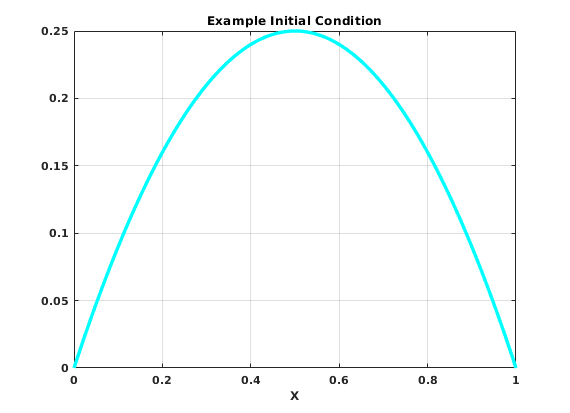
\includegraphics{lec23_ex1_smooth_ic.png}
\caption{Smooth initial condition.}
\label{fig:lec23-ex1-smooth-ic}
\end{marginfigure}

To build the solution we combine the eigenfunctions along with the coefficients calculated using Equation \ref{eq:lec23-ex1-coeff}.

\begin{lstlisting}[name=lec23_ex1, style=myMatlab]
%% Compute the solution
% initialize my series solution
u = @(x,t) 0;
for n = 1:N
    % essentially doing the sine-series half-wave expansion
    % compute the coefficient
    cn = (2/L)*integral(@(x) f(x).*F(x,n),0,L);
    
    % add the term to the series solution
    u = @(x,t) u(x,t) + cn*F(x,n).*G(t,n);
end

%% plot the result
figure(1)
plot(X,u(X,0),'-b',...
    X,u(X,0.1),'-.g',...
    X,u(X,0.5),'--r','linewidth',3);
title_str = sprintf('Heat Equation Example, N=%d',N);
title(title_str,'FontSize',16,'FontWeight','bold');
%title('Lecture #23 Example','fontsize',16,'fontweight','bold');
xlabel('X','fontsize',14,'fontweight','bold');
ylabel('u(X,t)','fontsize',14,'fontweight','bold');
grid on
set(gca,'fontsize',12,'fontweight','bold');
legend('t = 0','t = 0.1','t = 0.5');
\end{lstlisting}
\begin{marginfigure}
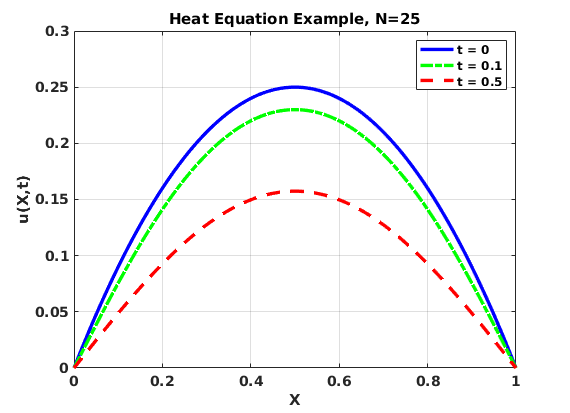
\includegraphics{lec23_ex1_smooth_ic_n25.png}
\caption{Solution for smooth initial condition.}
\label{fig:lec23-ex1-smooth-plot}
\end{marginfigure}
\newthought{The plot is shown} in Figure \ref{fig:lec23-ex1-smooth-plot}. As is expected, the temperature is going down over time. As time goes to infinity, the solution will be zero everywhere.  Recalling that the heat equation is simply a mathematical representation of conservation of energy, you should ask yourself the question: where is the energy going?  The answer is that the energy is flowing out of the left and right side of the bar and will continue to do so as long as the temperature of the bar is higher than the temperature at the boundary which, for this problem, is set to zero.

\newthought{What happens if} we increase the thermal diffusivity?  Answer: the heat flows ``faster.''  Since the thermal diffusivity shows up in the equation $G(t)$, the answer should look like time ``sped up.''  Testing this hypothesis out on our MATLAB solution, we change thermal diffusivity to 1.2.  The results are shown in Figure \ref{fig:lec23-ex1-smooth-plot-copper}.
\begin{marginfigure}
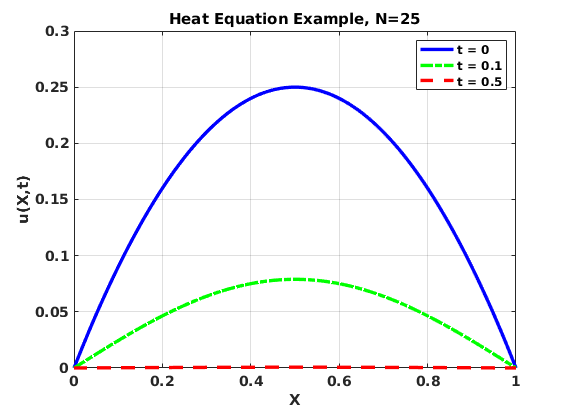
\includegraphics{lec23_ex1_smooth_ic_n25-copper.png}
\caption{Solution with high thermal diffusivity.}
\label{fig:lec23-ex1-smooth-plot-copper}
\end{marginfigure}

\newthought{What happens if} we have a much less smooth initial condition?  Admittedly, it would be odd for the initial temperature distribution to be discontinuous, but given our experience with Fourier series expansions, we should have some idea as to what the Fourier series expansions of discontinuous functions should look like.  To test this, suppose the initial temperature distribution were given by:
\begin{marginfigure}
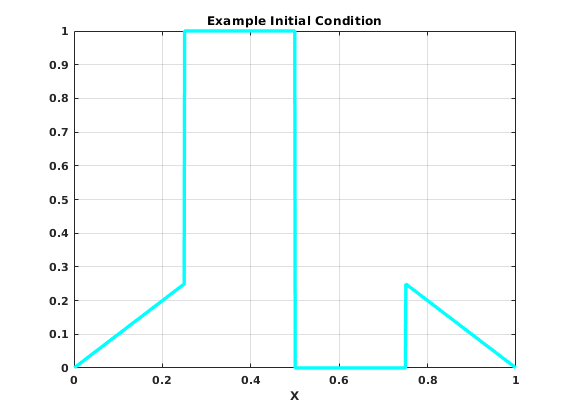
\includegraphics{lec23_ex1_discont_ic.png}
\caption{Example with discontinuous initial condition.}
\label{fig:lec23_ex1_discont}
\end{marginfigure}
\begin{equation*}
f(x) = 
\begin{cases}
x, & 0 < x < \frac{L}{4} \\
1, & \frac{L}{4} \le x < \frac{L}{2} \\
0, & \frac{L}{2} \le x < \frac{3L}{4} \\
L-x, & \frac{3L}{4} \le x < L

\end{cases}
\end{equation*}
and shown in Figure \ref{fig:lec23_ex1_discont}. The solution (for $\alpha^2=0.1$) is shown in Figure \ref{fig:lec23_ex1_discont_n25}. 
\begin{marginfigure} 
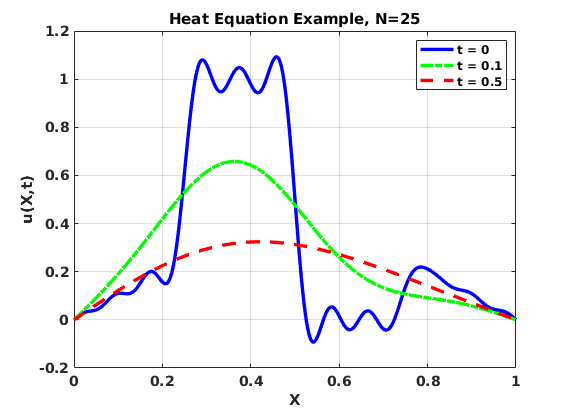
\includegraphics{lec23_ex1_discont_n25.png}
\caption{Solution with discontinuous initial condition, $N=25$.}
\label{fig:lec23_ex1_discont_n25}
\end{marginfigure} 
Note the ``wiggliness'' of the Fourier series representation of the initial condition; note also how that ``wiggliness'' goes away almost immediately.

In much the same way as we could improve our resolution of functions represented by a Fourier series by computing more terms, we can do the same thing here.  In Figure \ref{fig:lec23_ex1_discont_n100} we show the solution computed with $N=100$ terms in the Fourier series.
\begin{marginfigure}
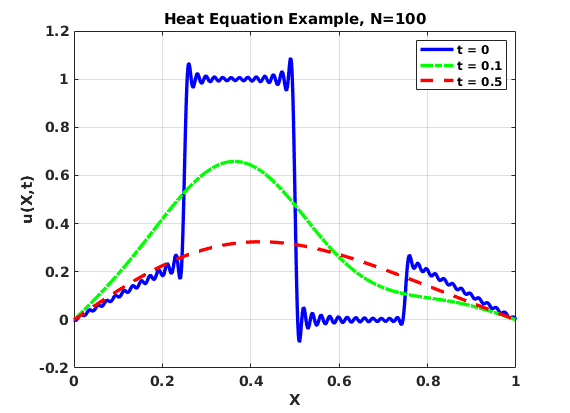
\includegraphics{lec23_ex1_discont_n100.png}
\caption{Solution with discontinuous initial condition, $N=100$.}
\label{fig:lec23_ex1_discont_n100}
\end{marginfigure}

\section{Insulated Boundaries}
%\subsection{One Boundary Insulated}
As an exercise, let us consider what happens when we change the problem by insulating the boundary at $x=L$.  

\begin{table}
\begin{tabular}{l l}
$\substack{\text{Governing} \\\text{Equation}}: $& $\frac{\partial u}{\partial t} = \alpha^2 \frac{\partial^2 u}{\partial x^2}, \ \ \alpha>0, \ \ 0<x<L, \ \ t>0$ \\
& \\
$\substack{\text{Boundary} \\ \text{Conditions}}: $& $u(0,t)=0, \ \ \frac{du}{dx}(L,t) = 0, \ \ t>0$\\
& \\
$\substack{\text{Initial} \\ \text{Conditions}}: $ & $u(x,0) = f(x), \ \ 0<x<L $ \\
\end{tabular}
\end{table}

\vspace{0.25cm}

\noindent Before we do any analysis we should think about what we \emph{expect} the solution to look like.  Mathematically we implement the insulated boundary condition by setting the temperature gradient at that boundary equal to zero.  Conceptually, we know this means that heat will no longer flow out of that boundary.  Heat may or may not flow \emph{towards} the right boundary depending on the temperature distribution within the domain but any heat reaching the right boundary will stay there until it can flow out towards the \emph{left} boundary.

\vspace{0.25cm}
\marginnote{\emph{Hint:} when we apply the insulated boundary condition, we will be left with $F_x(L) = \nu c_2 \cos{\nu L} = 0$ which we can satisfy if $\nu L$ is an odd integer multiple of $\sfrac{\pi}{2}$. So $\nu_n L = \frac{(2n-1) \pi}{2}, \ n=1,2,3,\cdots$, and therefore $\nu_n = \frac{(2n-1)\pi}{2L}$. 
}
\noindent The details are left to the reader but application of separation of variables to the new boundary value problem yields the following solution:

\begin{align*}
\nu_n &= \frac{(2n-1)\pi}{2L}, \ \ n=1,2,3,\dots \\
u(x,t) &= \sum\limits_{n=1}^{\infty} c_n \sin{\nu_n x}e^{-(\alpha \nu_n)^2 t} \\
c_n &= \frac{\int_0^L f(x) \sin{\nu_n x} \ dx}{\int_0^L \sin{(\nu_n x)}^2 \ dx}
\end{align*}
A plot of the solution when $N=25$, $L=1$, and $\alpha^2=1.5$ is shown in Figure \ref{fig:lec23-ex2-n25}.

\begin{marginfigure}
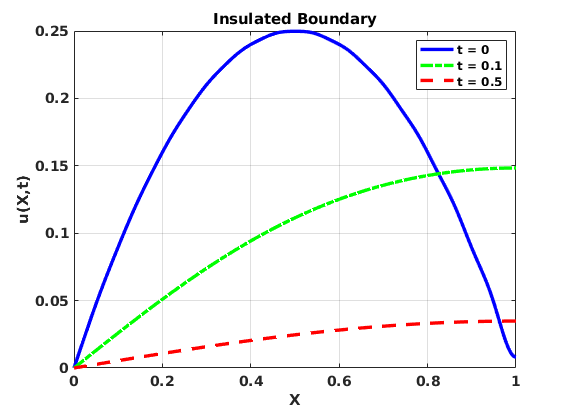
\includegraphics{lec23_ex2_smooth_n25_alphasq1p5.png}
\caption{Solution with an insulated boundary at $x=L$.}
\label{fig:lec23-ex2-n25}
\end{marginfigure}
%\subsection{Both Boundaries Insulated}

\newthought{What happens if} both boundaries are insulated?  Physically, when we insulate something, that means we want to keep heat from coming in or out of the domain.  Does this mean heat will not diffuse \emph{within} the domain?  Of course not; heat will simply flow as it must while driven by temperature gradients in the domain.  When will it stop?  When there is no more temperature gradient to drive heat flow and that will happen when the temperature is uniform.  

Mathematically, this means that we again change the boundary conditions so that the temperature gradient is zero at \emph{both} boundaries.  The details of this solution will be left to exercises but it is hoped by this point that you already know what the solution \emph{must} look like; namely that heat will diffuse within the domain until a uniform temperature is reached that is equal to the \emph{average} initial temperature.
